\documentclass{../source/Experiment}

\major{信息工程}
\name{姚桂涛}
\title{边界追踪}
\stuid{3190105597}
\college{信息与电子工程学院}
\date{\today}
\lab{}
\course{数字图像处理}
\instructor{李东晓}
\grades{}
\expname{边界追踪}
\exptype{设计验证}
\partner{}
\begin{document}
    \makecover
    \section{实验任务}

        本次选择的是PROJECT-10-02题目。

        \begin{enumerate}
            \item 编写一个基于 Moore 边界跟踪算法的边界跟踪程序,这里我们使得被跟踪得边界通过图像得方式输出。
            \item 下载图 9.14 来应用算法。
        \end{enumerate}

    \section{算法设计}
        算法实现如下:

        \begin{enumerate}
            \item 找到一个黑色像素,并将它定为你的起始像素。
            \item 每次遇到黑色像素,将设置为当前边界像素点
            \item 然后原路返回到先前到达的白色像素,以顺时针方向搜索的摩尔邻域内的每一个像素,直到遇到下一
            个黑色像素。
            \item 重复这个过程,当起始像素被第二次访问时算法终止,在整个运行过程走过的�色像素就是目标的边
            界像素。
        \end{enumerate}


    \section{代码实现}
        本次实验编程语言选择的是Matlab。

        \lstinputlisting[
            language  =   matlab
            ]{第六次/main.m}

    \section{实验结果}
        实验结果如下:

        \begin{figure}[H]
            \centering
            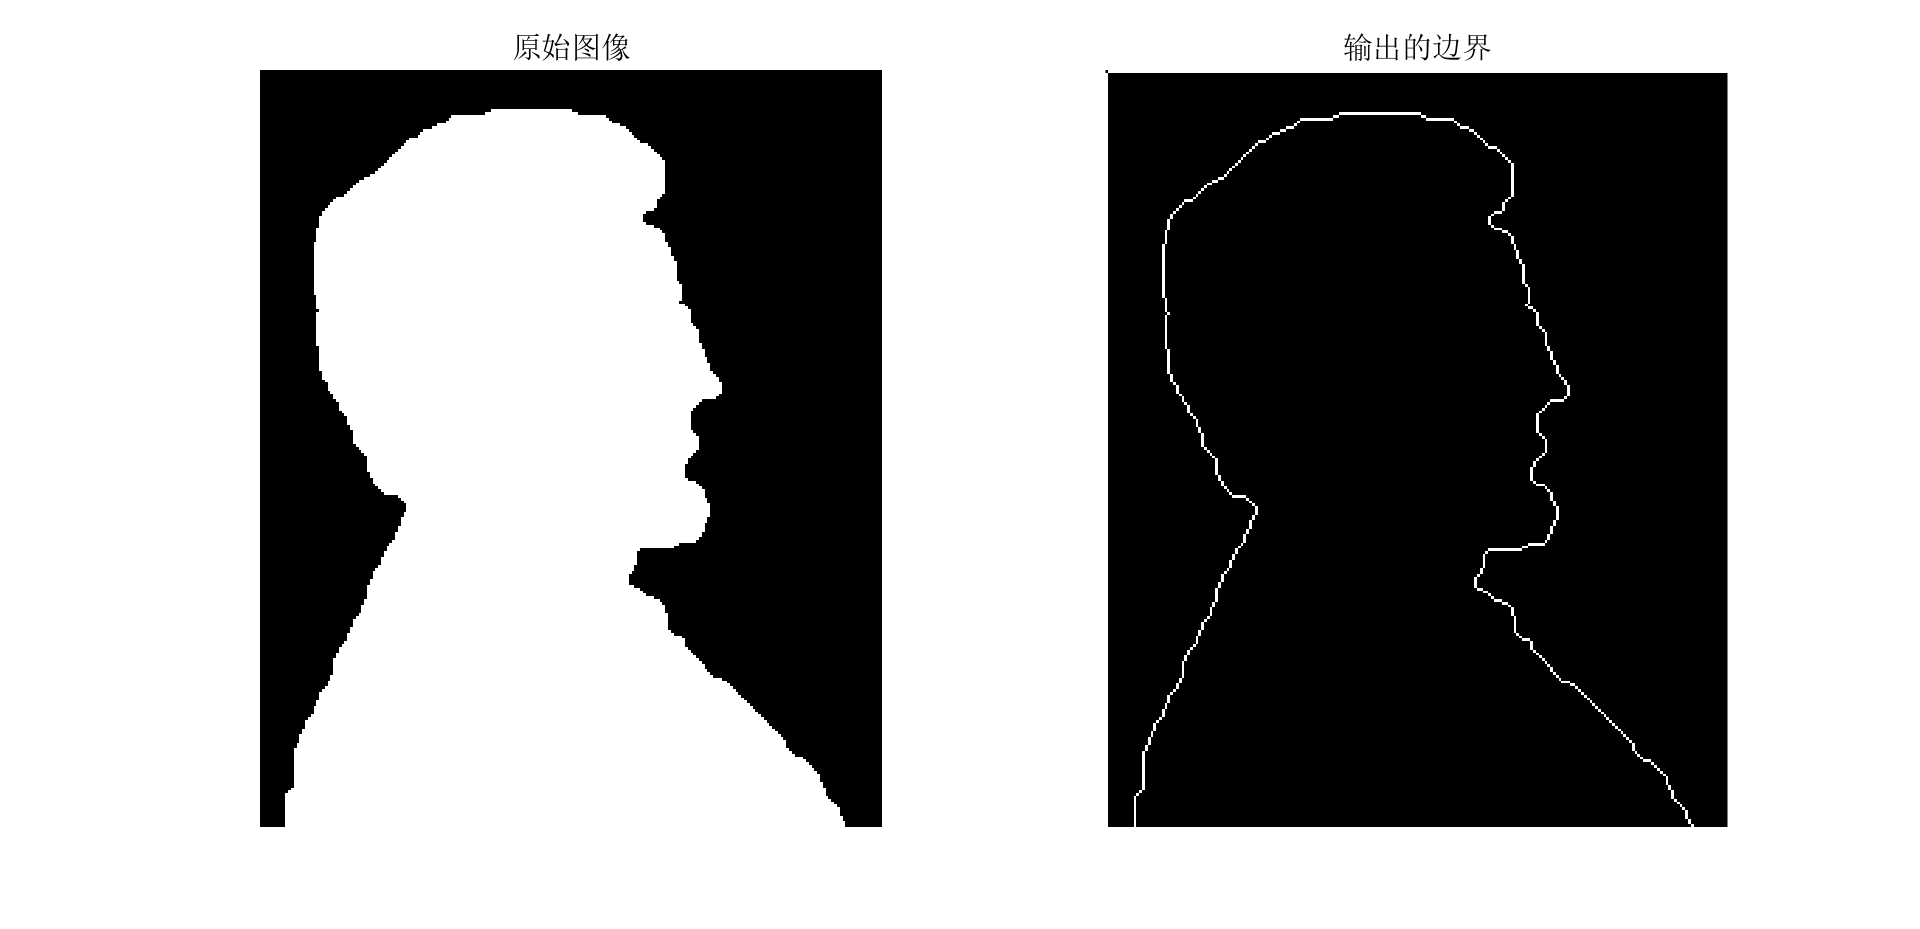
\includegraphics[width = 0.8\textwidth]{第六次/untitled.png}
        \end{figure}


    \section{总结}
    本次实验主要是通过Matlab编程语言实现了课程中所讲过的Moore算法跟踪边界原理。

    通过本次实验我对 Moore 算法图像边界跟踪更深的理解。

\end{document}



